\chapter{Security and Authorization Architecture}
\label{ch:security}

\section{Security Goals}

\noindent The security goals of the platform are: (i) tenant isolation that
holds at the enforcement layers by default; (ii) session security that resists
token theft and replay; (iii) authorization that evaluates current database
state instead of cached claims; and (iv) a contained attack surface in which
nothing user-facing depends on a publicly reachable internal service.

\section{Authentication}

\sectionmark{Authentication}
\noindent Authentication is cookie-based, following the OWASP guidance for
session management~\cite{owaspsession}. The flow is shown in
Figure~\ref{fig:auth-sequence}.

\begin{figure}[h]
\centering
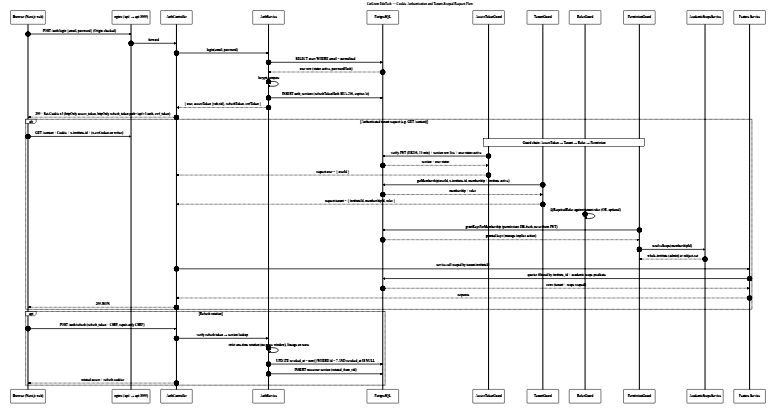
\includegraphics[width=\textwidth]{figures/authentication-sequence-bw.png}
\caption{Cookie authentication and the tenant-scoped request flow.}
\label{fig:auth-sequence}
\end{figure}

\subsection{Cookies and tokens}

\noindent Three cookies are issued:

\begin{itemize}
  \item \texttt{access\_token} --- httpOnly, path \texttt{/}, short-lived
  (default 15 minutes). It is a JWT, signed HS256, whose payload carries only
  \texttt{\{sub, sid\}}: the subject (user id) and the session id. Permissions
  are never placed in the token.
  \item \texttt{refresh\_token} --- httpOnly, path \texttt{/api/v1/auth},
  long-lived (default 30 days, sliding). Only its SHA-256 hash is stored in
  \texttt{auth\_sessions}.
  \item \texttt{csrf\_token} --- not httpOnly, path \texttt{/}, for the
  double-submit CSRF scheme.
\end{itemize}

\noindent SameSite defaults to \texttt{lax}; the \texttt{Secure} attribute is
enabled in production. In production the \texttt{JWT\_SECRET} must be present
at boot or the service refuses to start.

\subsection{Access token validation}

\noindent The \texttt{AccessTokenGuard} verifies the JWT, requires a
\texttt{sid}, loads the referenced \texttt{auth\_sessions} row, and checks that
the session is live (not revoked, not expired, owned by \texttt{sub}) and that
the user's status is still \texttt{active}. Revocation or deactivation
therefore takes effect on the very next request; there is no residual window.

\subsection{Strict refresh rotation}

\noindent Refresh rotation is strictly one-time. On \texttt{POST}
\texttt{/auth/refresh} the service atomically claims the session with
\texttt{UPDATE auth\_sessions SET revoked\_at = now() WHERE id = ? AND
revoked\_at IS NULL AND refresh\_token\_hash = ?}; only the single winning
request mints the successor row. There is no grace window --- re-rotation of a
spent token is treated as replay. If a spent token is presented, the service
walks the \texttt{rotated\_from\_sid} lineage and revokes the whole family; a
wrong token against a live row is treated as suspected theft and revokes that
session. \texttt{POST /auth/refresh} is also CSRF-guarded and CSRF-repair-only.
Logout is refresh-session aware: it revokes by the refresh session id first,
falls back to the access \texttt{sid} claim, and clears the cookies
unconditionally. Users may list their sessions and revoke any single one or
all but the current session.

\subsection{CSRF protection}

\noindent The double-submit scheme is registered as a global guard. On every
state-changing (non-GET), cookie-authenticated request, the client must echo
the \texttt{csrf\_token} cookie in the \texttt{x-csrf-token} header; a
missing or mismatched value yields \texttt{403}. Requests without an access
cookie are exempt (there is no session to protect --- this is also the seam
that lets cookie-free worker protocols operate), and GET/HEAD/OPTIONS are
always allowed. The custom \texttt{x-institute-id} header doubles as
defense-in-depth, since cross-origin calls must pass browser CORS
preflight to send it.

\subsection{Login protection}

\noindent \texttt{POST /auth/login} is throttled (5 per 60 seconds), rejects
sessions for deactivated accounts, returns uniform responses that do not
enumerate users, and validates that the request Origin matches the Host.
Passwords are hashed with bcrypt (cost~12 for new accounts).

\subsection{Password reset}

\noindent The reset flow issues a one-time token (identifier plus a 32-byte
secret), stores only the bcrypt hash of the secret, expires it after 30
minutes, and atomically consumes it via a \texttt{used\_at} guard. A
successful reset revokes every session of the user. Delivery of the reset
token is an integration seam (provider not yet wired), and the raw token is
never logged.

\section{Authorization}

\noindent Authorization is evaluated per request and in layers. The complete
decision chain is rendered in Figure~\ref{fig:permission-model};
the academic-scope engine is detailed in Figure~\ref{fig:academic-scope}.

\begin{figure}[h]
\centering
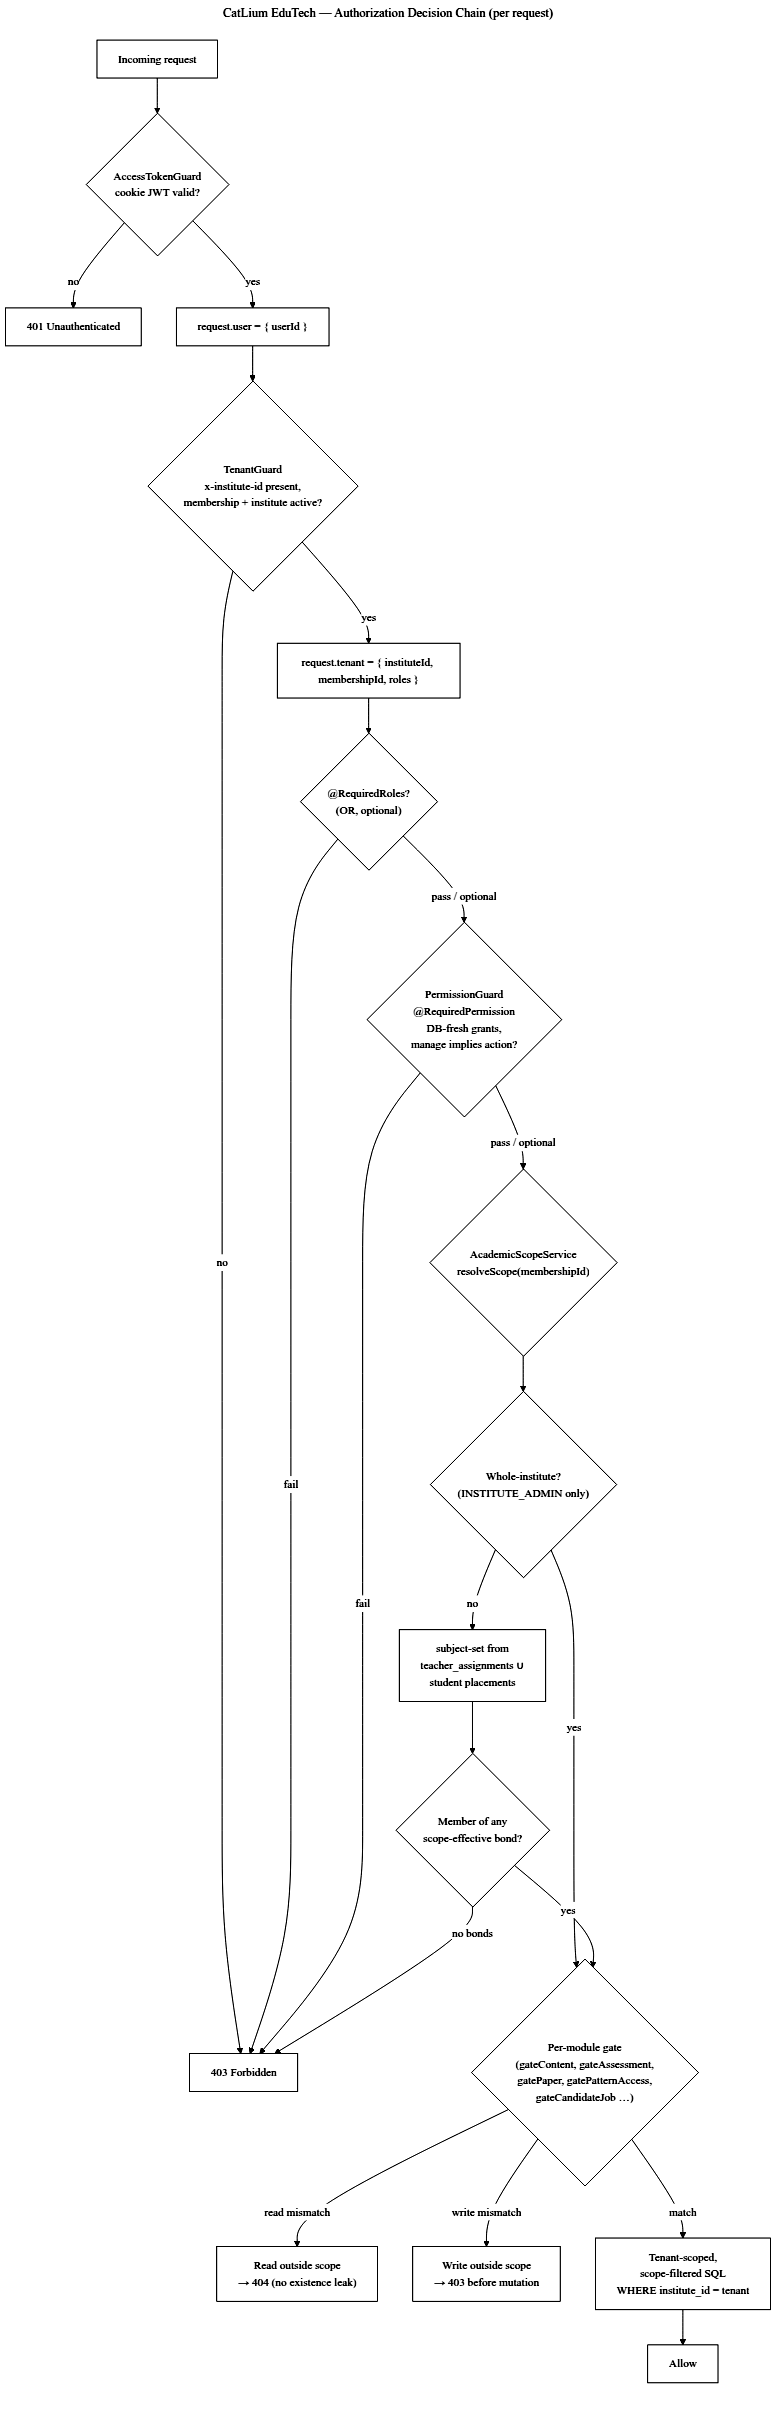
\includegraphics[width=\textwidth]{figures/permission-model-bw.png}
\caption{Authorization decision chain for a tenant-scoped request.}
\label{fig:permission-model}
\end{figure}

\begin{figure}[h]
\centering
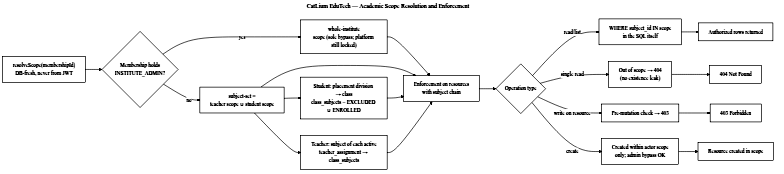
\includegraphics[width=\textwidth]{figures/academic-scope-bw.png}
\caption{Academic scope resolution and enforcement (reads 404, writes 403).}
\label{fig:academic-scope}
\end{figure}

\subsection{The guard chain}

\noindent For tenant-scoped endpoints the chain is
\texttt{AccessTokenGuard} $\rightarrow$ \texttt{TenantGuard} $\rightarrow$
\texttt{RolesGuard} $\rightarrow$ \texttt{PermissionGuard}. Public endpoints
and the platform plane use
lighter chains (see below). A permission check is
\emph{DB-fresh}: the \texttt{PermissionGuard} loads the membership's granted
keys by joining memberships $\rightarrow$ roles $\rightarrow$ role permissions
$\rightarrow$ permissions and evaluates against the declared
\texttt{@RequiredPermission} keys; \texttt{R.manage} implies any action of
resource \texttt{R}. Nothing about authorization is cached across requests,
so removing a role or permission takes effect on the next request.

\subsection{The permission catalogue}

\noindent The catalogue is a single typed map in code (mirrored into the
\texttt{permissions} table at every API boot) with 83 keys over 19 resources.
Institute-domain resources \texttt{subjects}, \texttt{chapters},
\texttt{topics}, \texttt{content}, \texttt{materials}, \texttt{syllabus},
\texttt{questions}, \texttt{question-types}, \texttt{paper-patterns},
\texttt{question-papers}, \texttt{assessments}, \texttt{attempts},
\texttt{practice}, \texttt{exports}, \texttt{jobs}, \texttt{users}, and
\texttt{roles} each carry the actions \texttt{read}, \texttt{create},
\texttt{update}, \texttt{delete} (where an endpoint exists), and
\texttt{manage}; the platform domain carries \texttt{institutes} and
\texttt{ocr-workers}. Keys are explicit and without wildcards; unknown keys
resolve to \texttt{false}. The full catalogue is reproduced in
Appendix~\ref{app:permissions}.

\subsection{Built-in roles}

\begin{itemize}
  \item \texttt{INSTITUTE\_ADMIN} holds \texttt{manage} on every institute
  resource (17 keys) and resolves to whole-institute academic scope;
  \item \texttt{TEACHER} holds 47 institute keys covering content,
  materials, structure, questions, patterns, papers, assessments, reads on
  attempts, and job management;
  \item \texttt{STUDENT} holds 14 read-oriented keys over structure, content,
  syllabi, and assessments plus attempt/practice self-actions;
  \item \texttt{SUPER\_ADMIN} holds all nine platform keys and is never a
  membership role; the platform plane is enforced by \texttt{PlatformGuard},
  which is independent of \texttt{x-institute-id}.
\end{itemize}

\noindent Institute admins create custom roles from the institute catalogue
(max 128 keys per role). Custom roles never receive platform permissions, and
an actor cannot modify a role they currently hold (self-escalation guard).

\subsection{Academic scope}

\noindent A permission alone never grants access: the resource's subject (or
its absence) must also match the actor's scope. The
\texttt{AcademicScopeService} resolves the actor's subject set from \emph{current
database state}: for teachers, the union of subjects over their active
\texttt{teacher\_assignments}; for students, the class-subject set of their
placement's division, minus \texttt{EXCLUDED} and plus \texttt{ENROLLED}
enrollments. An actor with no bonds gets an empty set (default deny).
\texttt{INSTITUTE\_ADMIN} is the sole whole-institute bypass and never escapes
the institute.

\subsection{Enforcement points and status codes}

\noindent Reads are scoped in the SQL itself: list queries filter by the
subject predicate, and a single-resource read out of scope returns
\texttt{404} (no existence leak). Writes perform an explicit resource check
\emph{before} mutation and return \texttt{403}. Ownership layers supplement
scope on DRAFT and PENDING resources (owner-and-admin-only until shared).
Module gate helpers (\texttt{gateContent}, \texttt{gateAssessment},
\texttt{gatePaper}, \texttt{gatePatternAccess}, \texttt{gateCandidateJob})
apply the same 404-read/403-write contract across their modules.

\section{Internal Service Authentication}

\noindent Internal HTTP calls use a shared \texttt{x-internal-api-key} header
(sent by the API to the OCR service when so configured). Distributed OCR
workers authenticate per worker: \texttt{x-worker-id} plus a bearer
\texttt{owr\_...} key whose SHA-256 hash is stored on the worker row and
compared in constant time. Workers call the AI gateway with a standard
\texttt{Authorization: Bearer} endpoint key. There is no direct cloud AI SDK
call from application code.

\section{Summary of Security Decisions}

\noindent The security and authorization design was settled in seven recorded
architectural decisions (D1--D7) and a session-hardening list (F1--F6), all
implemented and validated:

\begin{center}
\small
\begin{tabular}{@{}p{0.7cm}p{5.1cm}p{8.2cm}@{}}
\toprule
\textbf{Dec.} & \textbf{Decision} & \textbf{Implementation summary} \\
\midrule
D1 & Permission model & Explicit \texttt{resource.action} keys, default-deny,
\texttt{manage} implication, no wildcards, catalogue---table consistency check. \\
D2 & Role/permission storage & \texttt{roles}, \texttt{permissions},
\texttt{role\_permissions}, and \texttt{membership\_roles} relations with
schema CHECKs and partial unique indexes. \\
D3 & Platform plane & \texttt{SUPER\_ADMIN} via
\texttt{platform\_user\_roles}, disjoint from membership; \texttt{PlatformGuard}
independent of tenant header. \\
D4 & Academic structure & Years, classes, divisions, class--subject offerings;
offerings at class level. \\
D5 & Assignments & Teacher assignments and student placements at offering
granularity; no division-level subjects. \\
D6 & Resource scope & Subject chain (with optional offering-level scope in
design) + default-deny; admin bypass is the sole exception; ownership
stages O1--O3. \\
D7 & Session hardening & F1--F6: session-bound access tokens, strict one-time
rotation with lineage revocation, refresh-aware logout, global double-submit
CSRF with origin check, status-gated refresh, defined cookie and retention
posture. \\
\bottomrule
\end{tabular}
\end{center}

\noindent A documentation-led security audit (Phase~M) verified the
implementation against the threat model and remediated the findings: an export
endpoint that could expose answer keys was closed (HIGH), a cross-institute
OCR/enhancement job adoption path was fixed (MEDIUM), job ownership was
recorded (LOW), stale institute context was cleaned on logout (LOW), and
documentation was brought in line with the code.